\documentclass[11pt]{article}
\usepackage{fullpage}
\usepackage{graphics,epsfig,color}
\usepackage{wrapfig}

\usepackage{times}
\usepackage{setspace}
\usepackage{amsmath,amsthm,amssymb}
%\usepackage[ruled,vlined,linesnumbered]{algorithm2e}
\usepackage{qtree}
\usepackage{subfigure}
\usepackage{url}



%for code from latexdraw
%\usepackage[usenames,dvipsnames]{pstricks}
%\usepackage{epsfig}
%\usepackage{pst-grad} % For gradients
%\usepackage{pst-plot} % For axes


\newtheorem{theorem}{Theorem}[section]
%\newtheorem{proposition}{Proposition}[theorem]
\newtheorem{corollary}{Corollary}[section]
\newtheorem{lemma}{Lemma}[section]
%\newtheorem{claim}{Claim}[section]
\newtheorem{problem}{Problem}
%\newtheorem{conjecture}{Conjecture}[section]
\newtheorem{definition}{Definition}[section]
\newtheorem{observation}{Observation}[section]
\newtheorem{example}{Example}[section]
\newtheorem{openproblem}{Open Problem}[section]
\newtheorem{fact}{Fact}[section]
%\newcommand{\qedsymb}{\hfill{\rule{2mm}{2mm}}}

\newcommand{\qedsymb}{\hfill{\rule{2mm}{2mm}}}
\newenvironment{proofsketch}{\begin{trivlist}
\item[\hspace{\labelsep}{\noindent Proof Sketch: }]
}{\qedsymb\end{trivlist}}



%the following few lines until usepackage{algorithm2e} is to avoid the
%conflicts of algorithm2e with other packages.
\makeatletter
\newif\if@restonecol
\makeatother
\let\algorithm\relax
\let\endalgorithm\relax
%\usepackage[ruled,vlined,linesnumbered]{algorithm2e}
\usepackage[ruled,vlined,linesnumbered]{algorithm2e}


%\newenvironment{proof}{\begin{trivlist}
%\item[\hspace{\labelsep}{\bf\noindent Proof: }]}{\qedsymb\end{trivlist}}
%\newcommand{\qed}{\hfill\rule{2mm}{2mm}}

\newcommand{\remove}[1]{}



%--------------------------------


\begin{document}

\begin{center}
  {\LARGE CSCD501 Homework1}

\bigskip 

{\Large Will Czifro}

\end{center}

\bigskip

\noindent{\bf Solution for Problem prob:1.}

\begin{itemize}
\item The flow of this graph is 10
\item This is not a max flow. The max flow is 11. Consider Figure \ref{fig:maxFlow}
\item Consider Figure \ref{fig:residual}
\item Consider Figure \ref{fig:minCut}
\item In a max flow graph, one would see that $(d,b)$ and $(d,c)$ have no flow. In the residual graph of that max flow, those edges would have back edges showing that path $s \rightarrow d \rightarrow b$ and $s \rightarrow d \rightarrow c$ are not feasible. Thus we exclude these edges in summing the weight of the edges. The min cut then is 11, proving the original graph is not max flow.
\end{itemize}

%---------------------------------------
\bigskip

\noindent{\bf Solution for Problem prob:2.}

This is false. Consider Figure \ref{fig:maxFlow}. This graph has max flow, but $(s,a)$ is under saturated.

%---------------------------------------
\bigskip

\noindent{\bf Solution for Problem prob:3.}

This is false. Consider Figure \ref{fig:minCutSwitch}.

%---------------------------------------
\bigskip

\noindent{\bf Solution for Problem prob:4.}

Standard Form:

\begin{align*}
\quad & Maximize: d_t^\prime - d_t^{\prime\prime}\\
      & Constraints:\\
      & d_v^\prime - d_v^{\prime\prime} - d_u^\prime + d_u^{\prime\prime} \leq w(u,v), \quad for\;each\;(u,v) \in E\\
      & d_v^\prime \geq 0, \quad for\;each\;v \in V\\
      & d_v^{\prime\prime} \geq 0, \quad for\;each\;v \in V\\
      & d_s \geq 0\\
      & -d_s \geq 0
\end{align*}

%\newline
Slack Form:

\begin{align*}
\quad & Maximize: d_t^\prime - d_t^{\prime\prime}\\
      & Constraints:\\
      & x = d_u^\prime - d_u^{\prime\prime} + w(u,v) - d_v^\prime + d_v^{\prime\prime}, \quad for\;each\;(u,v) \in E\\
      & x \geq 0\\
      & d_s \geq 0\\
      & -d_s \geq 0\\
\end{align*}

%---------------------------------------
\bigskip

\noindent{\bf Solution for Problem prob:5.}

\begin{align*}
\quad & Maximize: DV\\
      & Constraints:\\
      & DU \leq DU^\prime + w(E)\\
      & d_s = 0\\
\end{align*}

%---------------------------------------

\newpage

\begin{figure}[h!]
\begin{center}
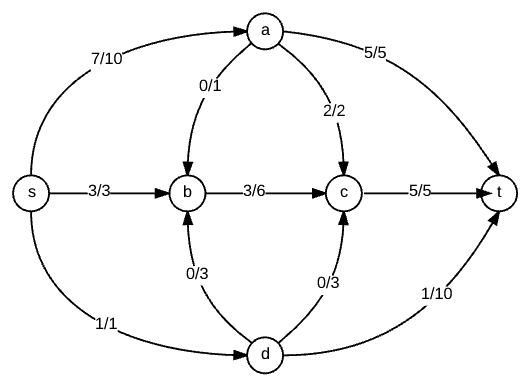
\includegraphics[scale=0.4]{MaxFlowGraph.png}
\caption{Max Flow}
\label{fig:maxFlow}
\end{center}
\end{figure}

\begin{figure}[h!]
\begin{center}
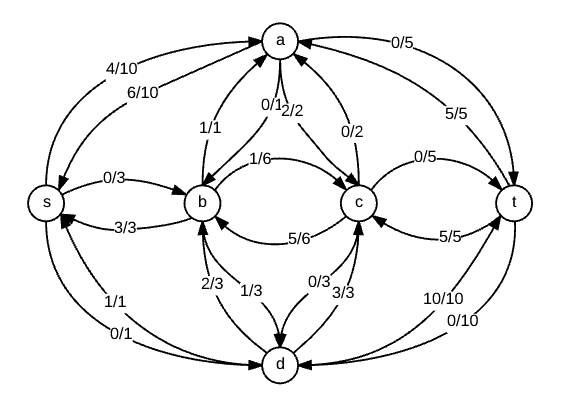
\includegraphics[scale=0.4]{ResidualGraph.png}
\caption{Residual Graph}
\label{fig:residual}
\end{center}
\end{figure}

\begin{figure}[h!]
\begin{center}
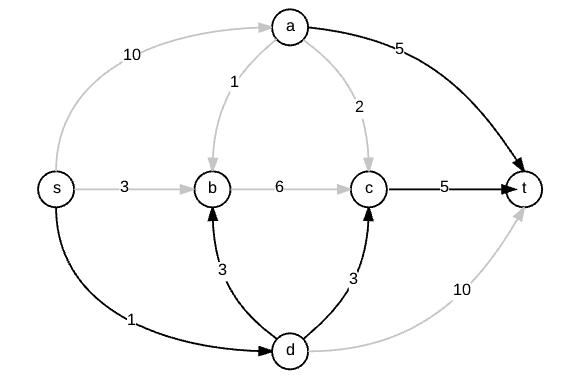
\includegraphics[scale=0.4]{MinCutGraph.png}
\caption{Min Cut}
\label{fig:minCut}
\end{center}
\end{figure}

\begin{figure}[h!]
\begin{center}
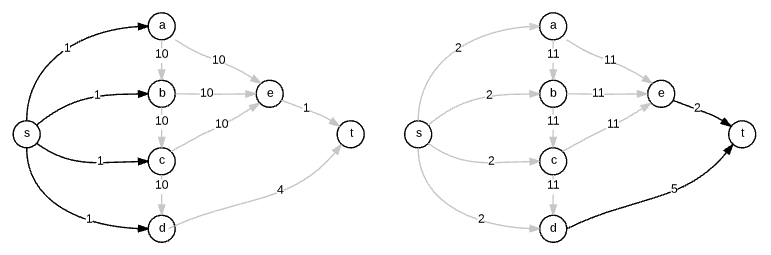
\includegraphics[scale=0.4]{MinCutSwitch.png}
\caption{Min Cut}
\label{fig:minCutSwitch}
\end{center}
\end{figure}


\end{document}




